
\documentclass{sig-alternate}

\usepackage{tikz}
\usetikzlibrary{shapes,arrows}

\begin{document}

% Define block styles
\tikzstyle{decision} = [diamond, draw, fill=blue!20, 
    text width=4.5em, text badly centered, node distance=3cm, inner sep=0pt]
\tikzstyle{block} = [rectangle, draw, fill=blue!20, 
    text width=6em, text centered, rounded corners, minimum height=4em]
\tikzstyle{goal_block} = [rectangle, draw, fill=blue!20, 
    text width=0.95\columnwidth, text centered, rounded corners, minimum height=4em]
\tikzstyle{process_block} = [rectangle, draw, fill=blue!20, 
    rounded corners]
\tikzstyle{line} = [draw, -latex']
\tikzstyle{cloud} = [draw, ellipse,fill=red!20, node distance=3cm,
    minimum height=2em]

\title{An Instructional Design Case Study for Computer Science Education}
\numberofauthors{1}
\author{
	\alignauthor {Austin Cory Bart, Eli Tilevich, Clifford A. Shaffer, Dennis Kafura}\\
	\email{\{acbart, tilevich, shaffer, kafura\}@vt.edu}\\
	\affaddr{Virginia Tech}  \\
}

\maketitle
\begin{abstract}
Abstract will go here
\end{abstract}

% A category with the (minimum) three required fields
\category{K.3.2}{Computer and Information Science Education}{Computer Science Education}

\terms{Design, Human Factors, Reliability, Experimentation}

\keywords{Instructional Design, Robert Gange, Dick \& Carey} % NOT required for Proceedings

\section{Introduction}

Instructional Design is the systematic design of effective Learning Experiences. 
Its history stretches back into the 1940s.

However, there has been few reported cases of its usage in Computer Science Education.

This paper describes a specific, popular Instructional Design model through a Computer Science Education case study.

\subsection{Roles}
An Instructional Designer is expected to be the advocate for the learner.
They are, first and foremost, dedicated to providing an optimal learning experience.
The instructional designer may or may not be responsible for actually physically teaching the learners (indeed, some instructional materials are designed without any physical instructor at all).

\subsection{Models of Instructional Design}

A number of competing models 
ADDIE
AGILE

\begin{figure*}
\begin{center}
	\begin{tikzpicture}[node distance = 2.5cm, auto]
			% Place nodes
			\node [block] (ig) {Instructional Goal};
			\node [block, above right of=ig] (ia) {Instructional Analysis};
			\node [block, below right of=ig] (lc) {Learner and Context Analysis};
			\node [block, below right of=ia] (po) {Performance Objectives};
			\node [block, right of=po] (ai) {Assessment Instruments};
			\node [block, right of=ai] (is) {Instructional Strategy};
			\node [block, right of=is] (im) {Instructional Materials};
			\node [block, right of=im] (fe) {Formative Evaluation};
			\node [block, below of=fe] (se) {Summative Evaluation};
			\node [block, above of=ai] (ri) {Revise Instruction};
			% Draw edges
			\path [line] (ig.north) |- (ia.west);
			\path [line] (ig.south) |- (lc.west);
			\path [line] (lc.east) -| (po.south);
			\path [line] (ia.east) -| (po.north);
			\path [line] (po.east) -- (ai.west);
			\path [line] (ai.east) -- (is.west);
			\path [line] (is.east) -- (im.west);
			\path [line] (im.east) -- (fe.west);
			\path [line] (fe.south) -- (se.north);
			\path [line] (fe.north) |- (ri.east);
			\path [line, dashed] (ri.west) -| (ia.north);
			\path [line, dashed] (ri.west) -| (po.north);
			\path [line, dashed] (ri.south) -| (ai.north);
			\path [line, dashed] (ri.south) -| (is.north);
			\path [line, dashed] (ri.south) -| (im.north);
			%\path [line] (identify) -- (evaluate);
			%\path [line] (evaluate) -- (decide);
			%\path [line] (decide) -| node [near start] {yes} (update);
			%\path [line] (update) |- (identify);
			%\path [line] (decide) -- node {no}(stop);
			%\path [line,dashed] (ia) -- (ig);
			%\path [line,dashed] (lc) -- (ig);
			%\path [line,dashed] (lc) |- (evaluate);
	\end{tikzpicture}
	\caption{The Dick \& Carey Model of Instructional Design}
	\label{dick-carey-overview}
\end{center}
\end{figure*}

In this case study, we use the Dick \& Carey model of Instructional Design, originally published in 1978 but continually updated and refined since then.
Figure \ref{dick-carey-overview} gives an overview of this model.
The model is meant to be iterative.

%http://delivery.acm.org.ezproxy.lib.vt.edu/10.1145/1160000/1151596/p41-east.pdf?ip=128.173.127.127&id=1151596&acc=ACTIVE%20SERVICE&key=B33240AC40EC9E30%2E80AE0C8B3B97B250%2E4D4702B0C3E38B35%2E4D4702B0C3E38B35&CFID=650919337&CFTOKEN=97456003&__acm__=1435239969_2e413e7f69af34d044bfae7cb3720913

%http://delivery.acm.org.ezproxy.lib.vt.edu/10.1145/1290000/1288595/p111-caspersen.pdf?ip=128.173.127.127&id=1288595&acc=ACTIVE%20SERVICE&key=B33240AC40EC9E30%2E80AE0C8B3B97B250%2E4D4702B0C3E38B35%2E4D4702B0C3E38B35&CFID=650919337&CFTOKEN=97456003&__acm__=1435239847_0c792845f04d9cd59e557a2cb011434e

One of the most influential\cite{anglin1992reference} instructional theories is Gang\'{e}'s Theory of Instruction, a complex Cognitivist model that categorizes different types of learning outcomes (e.g., ``Verbal Information'' such as reciting the definition of a term, ``Attitudinal'' such as choosing to not smoke) and breaks down the process of learning into nine coherent steps. Gang\'{e} stresses that different learning outcomes require very different instructional implementations of the general instructional model. This instructional theory informs the design of complete Instructional Design models such as the Dick and Carey model \cite{carey2001systematic}. Although different ID models suggest different approaches to creating instructional materials, those materials are all typically patterned after Gang\'{e}'s instructional events.

\section{The Case Study}

In this section, we will describe each phase of the D\&C model and our results using the model.
We took on the role of instructional designers to create new content for an introductory computing class on ``Computational Thinking'' for non-Computer Science majors.
The students in this course are expected to have no prior programming experience and are taking the course as part of the university's general requirements.
They come from many different disciplines, including the arts, sciences, engineering, agriculture, and more.
Because the curriculum is largely designed from scratch, there are many opportunities for instructional design.

When reviewing our results, keep in mind that the model is meant to be iterative, and any results we have generated are the result of several iterations. 
Any work presented is therefore neither completed nor prototypical.

\subsection{Identify Instructional Goal}

The first step in the Dick \& Carey Model is to identify the instructional goal(s) that you want to accomplish.
Critically, it does not describe anything about how the instructor will teach the material -- only what learners are expected to be able to do at the end of instruction.
This goal can come from a variety of sources.
The most obvious source is a department- or instructor- mandated curriculum, which may explicitly lay out what is expected of students.
Goals can also come from a perceived gap in learners existing ability.
In the full Dick \& Carey model, it is possible that instruction is not needed.
For instance, instead of teaching employees how to use complex software, the user interface of the software could be streamlined instead.
Because instructional design can be a very time and energy consuming process, it is important to find evidence (either quantitative or qualitative) of the need for instruction.

A complete goal statement should describe: the learners; the performance context; the action that learners should be able to do in the performance context; and the tools that are available to the learners in the performance context.
A major, common misstep in writing an instructional goal is to create a \textit{fuzzy goal}, usually describing an abstract, unobservable outcome using verbs such as ``appreciate'' or ``know''.
To correct a vague goal, the designer should begin by writing down the goal.
Then, they list examples of what people do to demonstrate that they have achieved this goal.
The designer can use this list to iteratively develop more concrete goals that will lead to observable outcomes.

In this case study, we wanted students to better understand variables and program state.
The instructors and teaching assistants of the course repeatedly mentioned this as one of the weakest areas for students, despite being one of the most important conceptually.
Many students struggled to write basic programs because of their inadequate understanding of how to use variables.
Our final goal statement is:

\textit{An Undergraduate, non-CS major} (\textbf{Learners})...\\
\textit{... Given source code} (\textbf{Performance Context}) ...\\
\textit{... Will be able to identify the name, value, origin, and type of a variable at any given step within the code} (\textbf{Action})... \\
\textit{... Taking advantage of any resources from the internet and their Integrated Debugging Environment} (\textbf{Tools}).

\subsection{Conduct Instructional Analysis}

The next step is conduct an Instructional Analysis, which will spell out exactly what the successful learner will do in the performance context.
Like the Instructional Goal, it does not describe how to teach the material, although it is easy for practice-oriented thinkers to accidentally start diagramming the lesson instead.
The Instructional Analysis first requires the designer to classify the goal statement based on the the kind of learning it requires.
Then, the designer identifies and organizes the \textit{subskills} involved in the skill being learned, and places them into an Instructional Analysis Diagram.

Dick \& Carey describe 4 learning outcomes, based on the work by Gagn\'{e}.
\textbf{Verbal Information} requires the simplest form of learning: it represents simple, declarative knowledge to be memorized and recalled (e.g., ``What is the worst-case runtime of the major sorting algorithms?'').
Very little presentation is usually needed for Verbal Information, although students may find it useful to practice such material.
\textbf{Intellectual Skills} are more complicated problem-solving tasks that demand some level of deeper cognition (e.g., ``Write a program to compute the sum of a list of numbers'').
Many types of knowledge in Computer Science require Intellectual Skills, but range greatly in complexity.
\textbf{Psychomotor Skills} are much rarer in Computer Science, describing the coordination of mental and physical activity (e.g., ``Type the alphabet using a keyboard'').
\textbf{Attitudes} is the fourth type, describing goals where the learner makes a choice (e.g., ``Choose to persevere in the face of segfaults'').
Gagn\'{e} also identified a fifth domain, \textbf{Cognitive Strategies}, but Dick \& Carey includes this as a particularly ill-structured form of Intellectual Skills.
Readers familiar with Bloom's Taxonomy will find these outcomes similar -- mappings exist between these lists, suggesting their rough equivalence.
It is up to the designer to choose their preferred schema.

\begin{figure*}
\begin{center}
	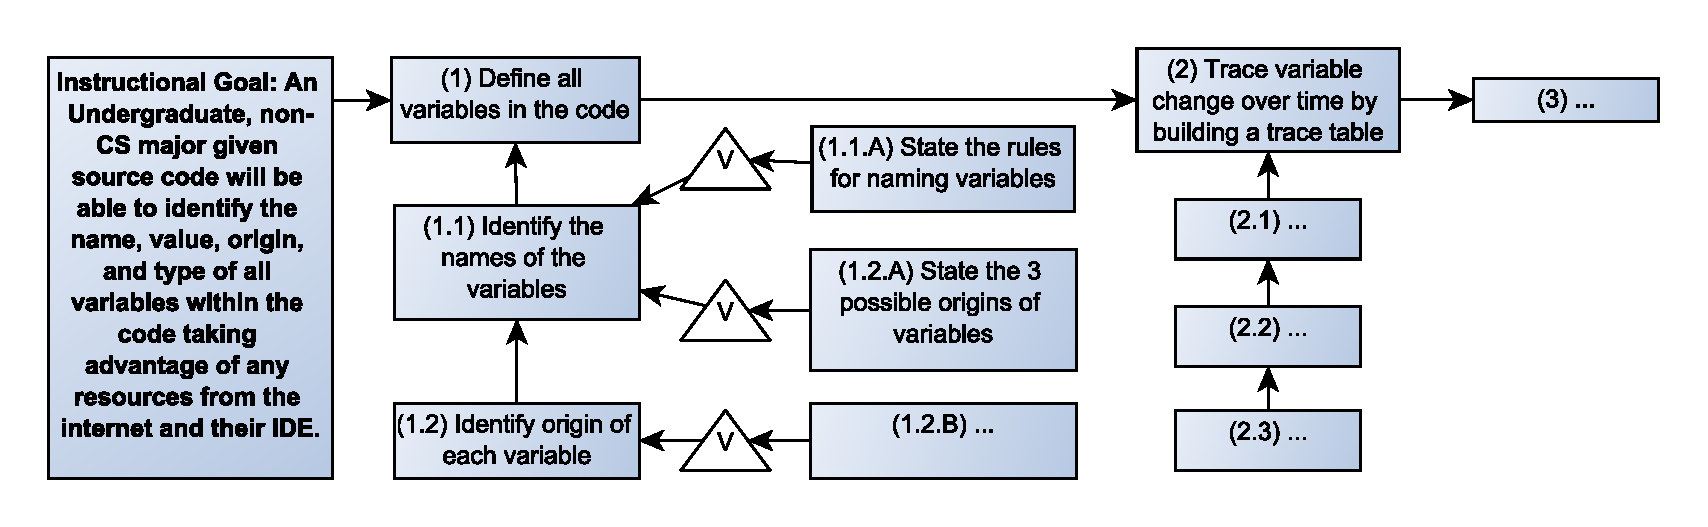
\psfig{file=images/ia_simple.eps, width=\linewidth}
	%\includegraphics[width=0.48\textwidth]{"images/rtw-client-library"}
\end{center}
\vspace{-\bigskipamount}
\caption{The Abridged Skill Analysis Diagram}
\label{fig-sa}
\end{figure*}

Once the goal is classified, the instructor performs a Subskill Analysis to concretely describe the goal and its components. 
Intellectual Skills and Psychomotor Skills is a typically straightforward process of creating a flowchart that breaks down each step into multiple levels.
Much as you would decompose the steps of a program, you decompose the skills into increasingly simpler steps.
Unlike a programming language, however, it is strictly up to the designer to decide when to terminate the iterative decomposition.
It is also possible to have branches and cycles, as is typical for flowcharts.
Some of the most basic subskills can be considered ``Entry Skills'' -- the learner can be expected to already have mastered them before the instruction begins.
These substeps might, in turn, involve Verbal Knowledge, which is denoted with a triangular ``V'' node.
Verbal Information is much simpler to diagram, although the designer can cluster the topics if they want;
in the runtime analysis example from before, for example, you might group the algorithms by their Big O values.
Attitudinal Skills can be considered a special form of the other skills: to resolve it, simply consider what skill the behavior in the goal is most akin to.

In this case study, our instructional goal is best classified as an Intellectual Skill.
Figure \ref{fig-sa} is an abridged version of the Instructional Analysis Diagram created for the goal.
The complete diagram is available in the online appendix.

\subsection{Conduct Learner and Context Analysis}

During the next phase, you will need to identify properties about the learners, the learning context, and the performance context. 
There are many factors involved in learner and context analysis.

Dick \& Carey suggest 8 crucial factors: (1) entry skills, (2) prior knowledge of the topic 
area, (3) attitudes toward content and potential delivery system, (4) academic 
motivation, (5) educational and ability levels, (6) general learning preferences, 
(7) attitudes toward the organization giving the instruction, and (8) group characteristics.

\subsection{Write Performance Objectives}

For every 
Writing performance objectives is a simple, but repetitive, phase.

\subsection{Develop Assessment Instruments}

There are four kinds of assessments.

\subsection{Develop Instructional Strategy}
As software developers, it is extremely tempting to 
\subsection{Develop and Select Instructional Materials}
Instructional Design Models such as Dick \& Carey usually delay the design of instructional materials till the end of the entire process, focusing initially on analysis of the learners, the performance context, the instructional goal, and a host of other critical factors. At that point, a content delivery system is chosen based on its educational affordances and suitability for the learning experience being developed. This delay reflects the typical role of an Instructional Designer as a \textit{consumer} of instructional technology -- they survey the available techniques and technology (e.g., traditional lecture, essay writing, websites), and choose the one that fits their need.

\subsubsection{Gagn\'{e}'s Instructional Events}

\begin{figure}
\begin{description}
	\item[(1) Gain Attention:] Stimulate the learner and motivate them to engage with the material.
	\item[(2) Describe Objectives:] Inform the learner will be able to do because of the instruction.
	\item[(3) Stimulating Recall of Prior Knowledge:] Remind students of their prior knowledge.
	\item[(4) Present the Material:] Using text, graphics, etc., give the instructional materials.
	\item[(5) Provide Guidance:] Give instructions on how to use the instructional materials.
	\item[(6) Elicit Performance:] Have the learners actively apply the new knowledge.
	\item[(7) Provide Feedback:] Show the learner what they did well and poorly on.
	\item[(8) Assess Performance:] Evaluate the learner on their performance
	\item[(9) Enhance Retention and Transfer:] Generalize the instruction by showing similar applications.
\end{description}
\caption{Gang\'{e}'s Nine Events of Instruction}
\label{gange-events}
\end{figure}

Gang\'{e}'s nine events are summarized in Figure \ref{gange-events}, taken indirectly from\cite{gagne1985conditions}. This model is described as an ordered, one-way sequence; however, in practice, some steps might be repeated and cycled between. For instance, very negative feedback might prompt the learner to return from step 7 to step 6. Modifications of the model have also been discussed in the literature. For example, to adapt for more Constructivist tastes, one could swap steps 4 and 6, so that students have the opportunity to engage with the materials before receiving instruction.


\subsection{Conduct Formative Evaluation}

\begin{figure}
\begin{tabular}{l|l|c|c|c}
	Phase & Student & Pretest & Posttest & Difference\\\hline
	1-1 & \#1 & 37.8\% & 100\% & +62.2\%\\
	1-1 & \#2 & 51.8\% & 100\% & +48.2\%\\
	1-1 & \#3 & 35.7\% & 84.6\% & +49.1\%\\\hline
	SG & \#1 & 21.7\% & 93.3\% & +71.6\%\\
	SG & \#2 & 54.6\% & 100\% & +45.4\%\\
	SG & \#3 & 64.3\% & 91\% & +26.7\%\\
	SG & \#4 & 32.7\% & 80\% & +47.3\%\\
	SG & \#5 & 69.4\% & 91\% & +21.6\%\\\hline
	& \textbf{Average} & 45.9\% & 92.5\% & +46.6\%\\
	& \textbf{StdDev} & 7.5\% & 16.6\% & 16.4\%\\
\end{tabular}
\caption{Student Performance during Formative Evaluation}
\label{fe-results}
\end{figure}

\subsection{Revise Instruction}
\subsection{Conduct Summative Evaluation}

\section{Conclusions}



\bibliographystyle{abbrv}
\bibliography{references} 

\end{document}
